\documentclass[aspectratio=169, table]{beamer}

\usepackage{colortbl}
\usepackage{xcolor}
\usepackage{listings}
\usepackage{pgfplots}
\usepgfplotslibrary{polar}
\usepackage{tikz}
\usetikzlibrary{shapes.geometric,
	positioning, shapes, shapes.multipart, backgrounds, arrows.meta, calc, fit, trees}

\usetheme{Pradita}

\lstdefinelanguage{yaml}{
    basicstyle=\ttfamily\scriptsize,
    keywordstyle=\color{blue}\bfseries,
    commentstyle=\color{gray}\itshape,
    stringstyle=\color{red},
    showstringspaces=false,
    breaklines=true,
    frame=lines,
    numbers=left,
    numberstyle=\tiny\color{gray},
    backgroundcolor=\color{lightgray!10},
    tabsize=2,
    morecomment=[l]{\#},
    literate=
      *{-}{{{\color{blue}\bfseries-}}}1
       {:}{{{\color{blue}\bfseries:}}}1
}

\lstdefinelanguage{bash} {
	keywords={},
	basicstyle=\ttfamily\scriptsize,
	keywordstyle=\color{blue}\bfseries,
	ndkeywords={iex},
	ndkeywordstyle=\color{purple}\bfseries,
	sensitive=true,
	commentstyle=\color{gray},
	stringstyle=\color{red},
	numbers=left,
	numberstyle=\tiny\color{gray},
	breaklines=true,
	frame=lines,
	backgroundcolor=\color{lightgray!10},
	tabsize=2,
	comment=[l]{\#},
	morecomment=[s]{/*}{*/},
	commentstyle=\color{gray}\ttfamily,
	stringstyle=\color{purple}\ttfamily,
	showstringspaces=false,
	captionpos=b
}

\lstdefinestyle{PythonStyle}{
    language=Python,
    basicstyle=\ttfamily\footnotesize,
    keywordstyle=\color{blue}\bfseries,
    commentstyle=\color{gray}\itshape,
    stringstyle=\color{red},
    showstringspaces=false,
    breaklines=true,
    frame=lines,
    numbers=left,
    numberstyle=\tiny\color{gray},
    backgroundcolor=\color{lightgray!10},
    tabsize=4,
    captionpos=b
}

\lstdefinelanguage{yaml}{
  keywords={true,false,null,yes,no},
  keywordstyle=\color{blue}\bfseries,
  sensitive=false,
  comment=[l]{\#},
  commentstyle=\color{gray}\ttfamily,
  stringstyle=\color{purple}\ttfamily,
  basicstyle=\ttfamily\scriptsize,
  numbers=left,
  numberstyle=\tiny\color{gray},
  breaklines=true,
  frame=lines,
  backgroundcolor=\color{lightgray!10},
  showstringspaces=false
}

\lstdefinelanguage{emfatic}{
  keywords={package,enum,class,abstract,attr,ref,val,extends},
  keywordstyle=\color{blue}\bfseries,
  sensitive=true,
  comment=[l]{//},
  commentstyle=\color{gray}\ttfamily,
  basicstyle=\ttfamily\scriptsize,
  numbers=left,
  numberstyle=\tiny\color{gray},
  breaklines=true,
  frame=lines,
  backgroundcolor=\color{lightgray!10},
  showstringspaces=false
}

\lstdefinelanguage{mediaflow}{
  keywords={graph,resource,scaler,transcoder,port,edge,from,to,backend,command,replicas,width,height,mediaType,uri,external},
  keywordstyle=\color{blue}\bfseries,
  sensitive=true,
  comment=[l]{\#},
  commentstyle=\color{gray}\ttfamily,
  stringstyle=\color{purple}\ttfamily,
  basicstyle=\ttfamily\scriptsize,
  numbers=left,
  numberstyle=\tiny\color{gray},
  breaklines=true,
  frame=lines,
  backgroundcolor=\color{lightgray!10},
  showstringspaces=false
}

\subtitle{IT30213 - Advanced Software Engineering \& DevOps}
\title{\Huge Model-Driven\vspace{8pt}\\
	Software Engineering}
\author{\textbf{Alfa Yohannis}}

\begin{document}

\frame{\titlepage}

\begin{frame}[fragile]
	\frametitle{Contents}
	\vspace{20pt}
	\begin{columns}[t]
		\column{0.5\textwidth}
		\tableofcontents[sections={1-5}]

		\column{0.5\textwidth}
		\tableofcontents[sections={6-20}]
	\end{columns}
\end{frame}

\begin{frame}{\hfill}
	\centering
	\Huge{\textbf{How can one metamodel support many media pipelines?}}
\end{frame}

\section{Tujuan Pembelajaran}
\begin{frame}{\hfill}
	\centering
	\Huge{\textbf{Tujuan Pembelajaran}}
\end{frame}

\begin{frame}{Tujuan Pembelajaran}
\vspace{6pt}
Setelah sesi ini, mahasiswa diharapkan mampu:
\begin{enumerate}
  \item Menjelaskan konsep inti \textit{Model-Driven Software Engineering} (MDSE): metamodel, model, instance, transformasi, dan validasi.
  \item Menganalisis relasi antara metamodel MediaFlow dan variasi model instance pipeline media.
  \item Membaca serta menyusun representasi model MediaFlow dalam bentuk tekstual (YAML/DSL) dan visual.
\end{enumerate}
\end{frame}

\section{Pendahuluan}
\begin{frame}{\hfill}
	\centering
	\Huge{\textbf{Pendahuluan}}
\end{frame}

\begin{frame}{Mengapa MDSE Penting?}
\vspace{6pt}
\begin{itemize}
  \item Kompleksitas sistem naik saat konfigurasi, komponen, dan variasi deployment bertambah.
  \item Pendekatan langsung di level implementasi sering memicu duplikasi dan inkonsistensi.
  \item MDSE menaikkan level abstraksi: fokus pada model domain sebagai artefak utama.
  \item Artefak implementasi diturunkan otomatis melalui aturan transformasi yang terkontrol.
  \item Dampak: proses lebih sistematis, mudah diaudit, dan lebih reproducible.
\end{itemize}
\end{frame}

\section{Konsep Dasar MDSE}
\begin{frame}{\hfill}
	\centering
	\Huge{\textbf{Konsep Dasar MDSE}}
\end{frame}

\begin{frame}{Metamodel, Model, dan Instance}
\vspace{8pt}
\begin{columns}[T]
\column{0.33\textwidth}
\textbf{Metamodel}
\begin{itemize}
  \item Aturan bentuk model valid.
  \item Mendefinisikan elemen, atribut, relasi.
\end{itemize}

\column{0.33\textwidth}
\textbf{Model}
\begin{itemize}
  \item Representasi sistem yang conform ke metamodel.
  \item Menyimpan keputusan desain domain.
\end{itemize}

\column{0.33\textwidth}
\textbf{Instance}
\begin{itemize}
  \item Realisasi konkret dari model.
  \item Menjadi data nyata atau artefak hasil transformasi.
\end{itemize}
\end{columns}
\end{frame}

\begin{frame}{Abstract Syntax dan Concrete Syntax}
\vspace{8pt}
\begin{columns}[T]
\column{0.5\textwidth}
\textbf{Abstract Syntax}
\begin{itemize}
  \item Struktur logis dan semantik model.
  \item Tidak terikat cara tampilan.
  \item Contoh: \texttt{subjek -> action -> objek}.
\end{itemize}

\column{0.5\textwidth}
\textbf{Concrete Syntax}
\begin{itemize}
  \item Bentuk presentasi model untuk manusia/tool.
  \item Visual: diagram.
  \item Tekstual: DSL, YAML, format deklaratif.
\end{itemize}
\end{columns}
\end{frame}

\begin{frame}{Transformasi dan Validasi dalam MDSE}
\vspace{4pt}
\centering
\scalebox{0.69}{
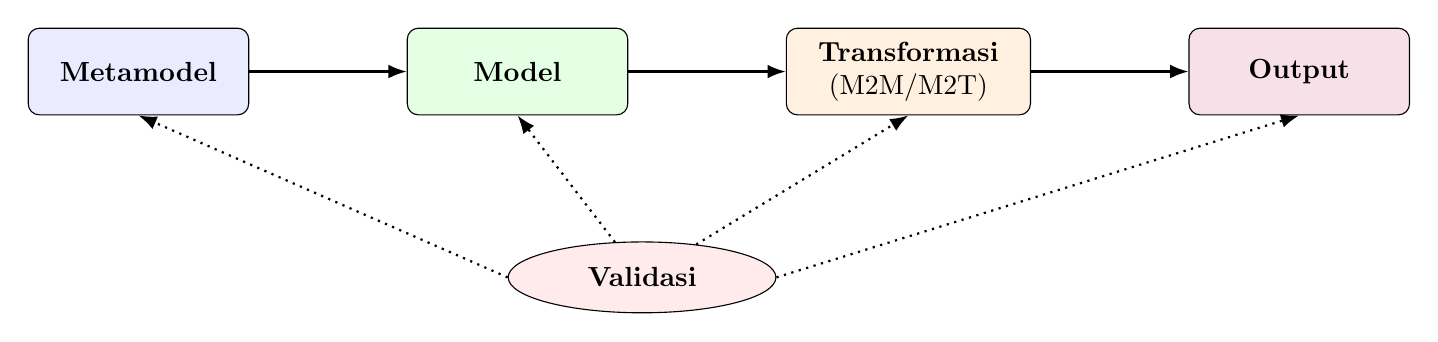
\begin{tikzpicture}[
  >=Latex,
  node distance=15mm and 20mm,
  box/.style={draw, rounded corners, minimum width=2.8cm, minimum height=1.1cm, align=center, fill=blue!8},
  box2/.style={draw, rounded corners, minimum width=2.8cm, minimum height=1.1cm, align=center, fill=green!10},
  box3/.style={draw, rounded corners, minimum width=3.1cm, minimum height=1.1cm, align=center, fill=orange!12},
  box4/.style={draw, rounded corners, minimum width=2.8cm, minimum height=1.1cm, align=center, fill=purple!12},
  val/.style={draw, ellipse, minimum width=3.4cm, minimum height=0.9cm, align=center, fill=red!8},
  arr/.style={->, thick}
]
  \node[box] (meta) {\textbf{Metamodel}};
  \node[box2, right=of meta] (model) {\textbf{Model}};
  \node[box3, right=of model] (trans) {\textbf{Transformasi}\\(M2M/M2T)};
  \node[box4, right=of trans] (inst) {\textbf{Output}};

  \node[val, below=16mm of model, xshift=45pt] (val) {\textbf{Validasi}};

  \draw[arr] (meta) -- (model);
  \draw[arr] (model) -- (trans);
  \draw[arr] (trans) -- (inst);

  \draw[arr, dotted] (val.west) -- (meta.south);
  \draw[arr, dotted] (val) -- (model.south);
  \draw[arr, dotted] (val) -- (trans.south);
  \draw[arr, dotted] (val.east) -- (inst.south);
\end{tikzpicture}
}

\vspace{6pt}
\small
M2M menghasilkan model target; M2T menghasilkan artefak tekstual seperti konfigurasi atau kode.
\end{frame}

\section{Contoh Konseptual SVO}
\begin{frame}{\hfill}
	\centering
	\Huge{\textbf{Contoh Konseptual SVO Lintas Bahasa}}
\end{frame}

\begin{frame}{Analogi SVO untuk Memahami Syntax}
\vspace{6pt}
\begin{itemize}
  \item Makna abstrak yang dijaga: \texttt{subjek -> action -> objek}.
  \item Bentuk konkret bisa berbeda antar bahasa, tetapi semantik tetap sama.
\end{itemize}

\vspace{8pt}
\begin{tabular}{|l|l|l|}
\hline
\textbf{Bahasa} & \textbf{Kalimat} & \textbf{Urutan Konkret} \\
\hline
Indonesia & Saya makan nasi & SVO \\
Inggris & I eat rice & SVO \\
Jepang & Watashi wa gohan o taberu & SOV \\
Tagalog & Kumakain ako ng kanin & VSO \\
\hline
\end{tabular}

\vspace{8pt}
\small
Ini merefleksikan konsep MDSE: \textit{abstract syntax} tetap, \textit{concrete syntax} bervariasi.
\end{frame}

\section{Ekosistem Tooling MDSE}
\begin{frame}{\hfill}
	\centering
	\Huge{\textbf{Ekosistem Tooling MDSE}}
\end{frame}

\begin{frame}{Tooling Utama di Praktik MDSE}
\vspace{4pt}
\begin{columns}[T]
\column{0.5\textwidth}
\textbf{Fondasi}
\begin{itemize}
  \item \textbf{Eclipse}: IDE untuk aktivitas modeling.
  \item \textbf{EMF}: framework metamodel, model, dan kode Java.
  \item \textbf{Ecore}: bahasa inti untuk struktur domain.
\end{itemize}

\column{0.5\textwidth}
\textbf{Lapisan Lanjutan}
\begin{itemize}
  \item \textbf{Emfatic}: sintaks tekstual ringkas untuk Ecore.
  \item \textbf{Epsilon}: validasi dan transformasi model.
  \item \textbf{Sirius}: editor visual berbasis metamodel.
\end{itemize}
\end{columns}

\vspace{8pt}
\small
Kombinasi tool ini membentuk alur end-to-end dari desain model hingga generasi artefak.
\end{frame}

\section{Studi Kasus MediaFlow}
\begin{frame}{\hfill}
	\centering
	\Huge{\textbf{Studi Kasus MediaFlow}}
\end{frame}

\begin{frame}{Apa itu MediaFlow?}
\vspace{6pt}
\begin{itemize}
  \item MediaFlow memodelkan alur pemrosesan media sebagai graf terarah.
  \item Fokus studi kasus: hubungan metamodel, model instance, validasi, dan representasi.
  \item Elemen domain utama: \texttt{Resource}, \texttt{Transformer}, \texttt{Port}, \texttt{Edge}.
  \item Pipeline dapat linear atau bercabang dengan struktur abstrak yang sama.
  \item Perubahan requirement dikelola pada level model, bukan hard-code workflow.
\end{itemize}
\end{frame}

\begin{frame}{Alur Pipeline pada MediaFlow}
\vspace{6pt}
\centering
\scalebox{0.72}{
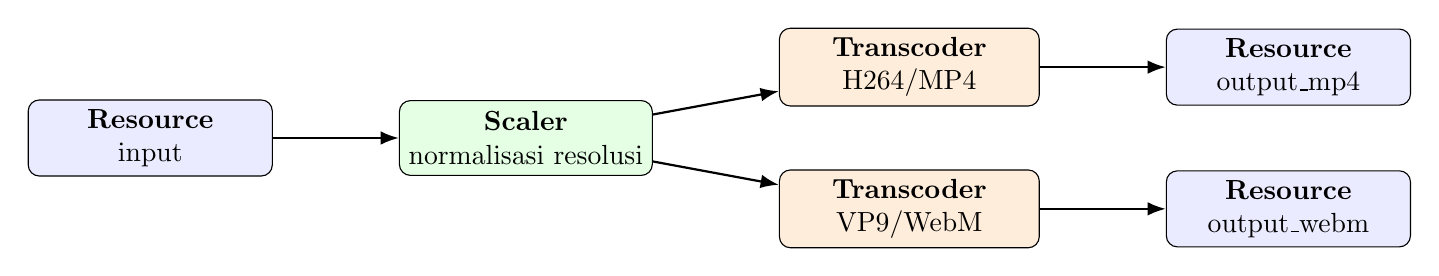
\begin{tikzpicture}[
  node distance=16mm and 16mm,
  >=Latex,
  res/.style={draw, rounded corners, minimum width=3.1cm, minimum height=0.95cm, align=center, fill=blue!8},
  scl/.style={draw, rounded corners, minimum width=3.2cm, minimum height=0.95cm, align=center, fill=green!10},
  trn/.style={draw, rounded corners, minimum width=3.3cm, minimum height=0.95cm, align=center, fill=orange!14},
  arr/.style={->, thick}
]
  \node[res] (input) {\textbf{Resource}\\input};
  \node[scl, right=of input] (scaler) {\textbf{Scaler}\\normalisasi resolusi};
  \node[trn, right=of scaler, yshift=9mm] (h264) {\textbf{Transcoder}\\H264/MP4};
  \node[trn, right=of scaler, yshift=-9mm] (vp9) {\textbf{Transcoder}\\VP9/WebM};
  \node[res, right=of h264] (out1) {\textbf{Resource}\\output\_mp4};
  \node[res, right=of vp9] (out2) {\textbf{Resource}\\output\_webm};

  \draw[arr] (input) -- (scaler);
  \draw[arr] (scaler) -- (h264);
  \draw[arr] (scaler) -- (vp9);
  \draw[arr] (h264) -- (out1);
  \draw[arr] (vp9) -- (out2);
\end{tikzpicture}
}
\end{frame}

\section{Metamodel MediaFlow}
\begin{frame}{\hfill}
	\centering
	\Huge{\textbf{Metamodel MediaFlow}}
\end{frame}

\begin{frame}{}
\centering
\begin{columns}[T]
\column{0.4\textwidth}
\vspace{30pt}
\textbf{Metamodel MediaFlow}
\begin{itemize}
\item Elemen utama:
\begin{itemize}
\item \texttt{Graph}
\item \texttt{Node}
\item \texttt{Edge}
\end{itemize}
\item Node terdiri dari:
\begin{itemize}
\item \texttt{Resource}
\item \texttt{Transformer}
\end{itemize}
\item Spesialisasi Transformer:
\begin{itemize}
\item \texttt{Scaler}
\item \texttt{Transcoder}
\end{itemize}
\item Edge menghubungkan output dan input antar node
\end{itemize}

\column{0.63\textwidth}
\vspace{-14pt}
\begin{figure}
\centering
\colorbox{white}{
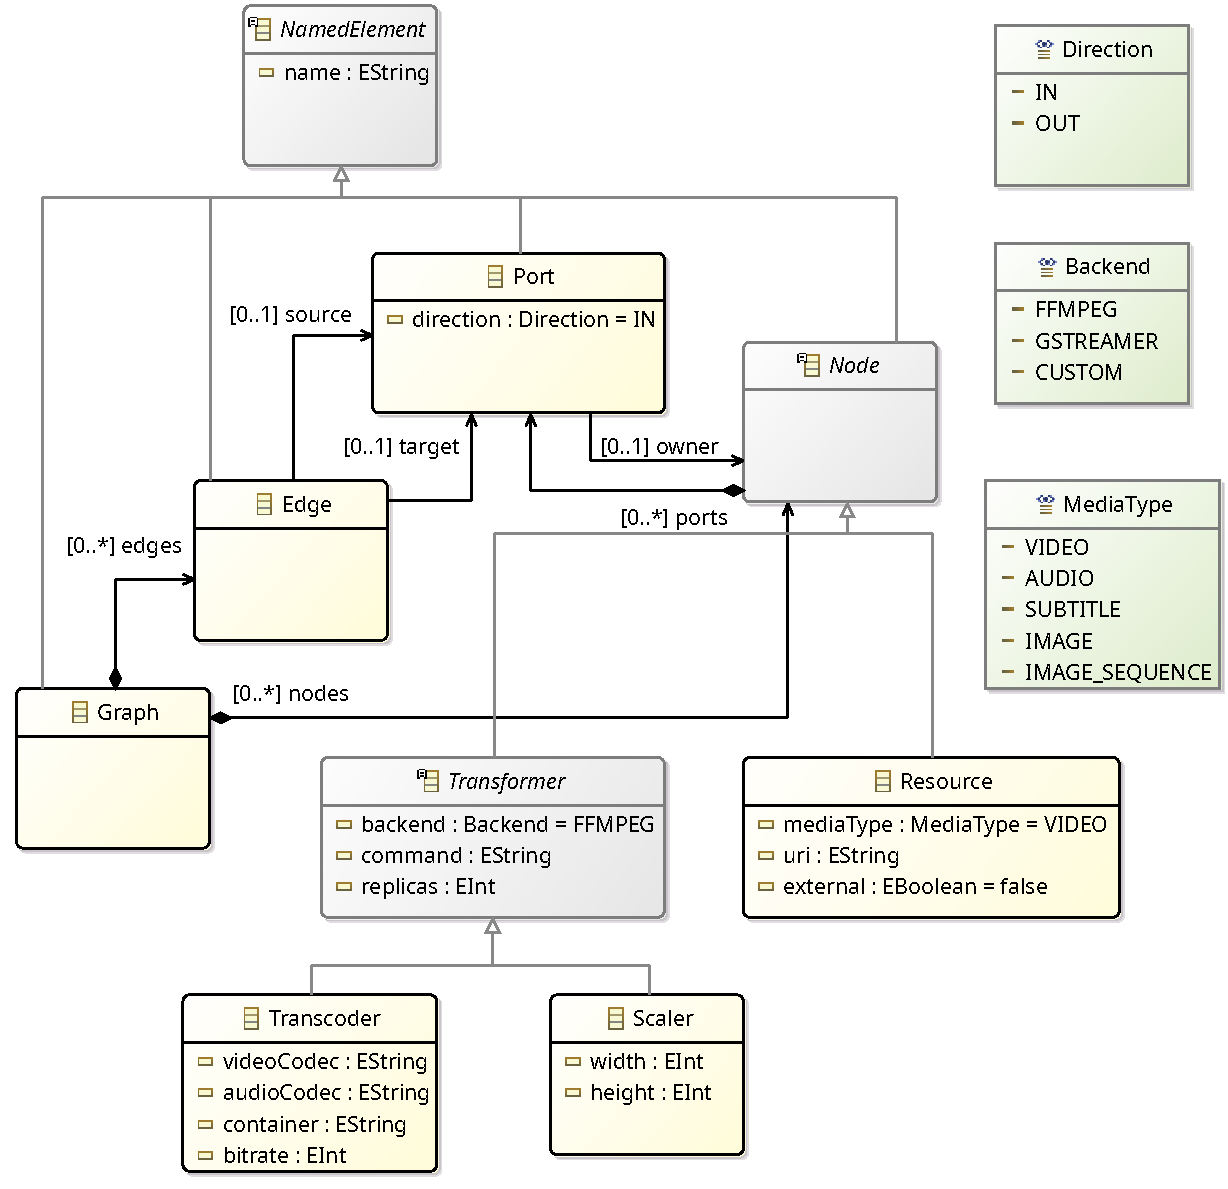
\includegraphics[width=\textwidth]{../../figures/mediaflow_class_diagram_cropped.pdf}
}
\label{fig:mediaflow-metamodel-class-diagram}
\end{figure}

\end{columns}

\end{frame}


\begin{frame}[fragile]{Contoh Definisi Emfatic Metamodel 1/2}
\vspace{20pt}
\begin{columns}[T]

\column{0.45\textwidth}

\begin{lstlisting}[language=emfatic, basicstyle=\ttfamily\scriptsize]
@namespace(uri="mediaflow", prefix="mediaflow")

package mediaflow;

enum MediaType {
  VIDEO = 1;
  AUDIO = 2;
  SUBTITLE = 3;
  IMAGE = 4;
  IMAGE_SEQUENCE = 5;
}

enum Backend {
  FFMPEG;
  GSTREAMER;
  CUSTOM;
}

\end{lstlisting}

\column{0.55\textwidth}

\begin{lstlisting}[language=emfatic, basicstyle=\ttfamily\scriptsize, firstnumber=18]
enum Direction {
  IN;
  OUT;
}

abstract class NamedElement {
  attr String name;
}

class Graph extends NamedElement {
  val Node[*] nodes;
  val Edge[*] edges;
}

abstract class Node extends NamedElement {
  val Port[*] ports;
}
\end{lstlisting}

\end{columns}

\end{frame}

\begin{frame}[fragile]{Contoh Definisi Emfatic Metamodel 2/2}
\vspace{20pt}
\begin{columns}[T]

\column{0.5\textwidth}

\begin{lstlisting}[language=emfatic, basicstyle=\ttfamily\scriptsize, firstnumber=35]
class Resource extends Node {
  attr MediaType mediaType;
  attr String uri;
  attr boolean external;
}

abstract class Transformer
      extends Node {
  attr Backend backend;
  attr String command;
  attr int replicas;
}

class Scaler extends Transformer {
  attr int width;
  attr int height;
}
\end{lstlisting}

\column{0.5\textwidth}

\begin{lstlisting}[language=emfatic, basicstyle=\ttfamily\scriptsize, firstnumber=51]
class Transcoder extends
      Transformer {
  attr String videoCodec;
  attr String audioCodec;
  attr String container;
  attr int bitrate;
}

class Port extends NamedElement {
  attr Direction direction;
  ref Node owner;
}

class Edge extends NamedElement {
  ref Port source;
  ref Port target;
}
\end{lstlisting}

\end{columns}

\end{frame}

\section{Model Instance MediaFlow}
\begin{frame}{\hfill}
	\centering
	\Huge{\textbf{Model Instance MediaFlow}}
\end{frame}

\begin{frame}[fragile]{Model 1: Pipeline Linear (\texttt{flow1.model})}
\vspace{4pt}
\begin{lstlisting}[language=yaml]
graph: flow1
nodes:
  - type: Resource
    name: input_video
    external: true
  - type: Scaler
    name: scaler_720
    command: scale=1080:720
    replicas: 1
  - type: Resource
    name: output_video
    external: true
edges:
  - source: input_video_out
    target: scaler_720_video_in
  - source: scaler_720_video_out
    target: output_video_in
\end{lstlisting}
\end{frame}

\begin{frame}[fragile]{Model 2: Pipeline Bercabang (\texttt{flow2.model})}

\begin{columns}[T]

\column{0.6\textwidth}

\begin{lstlisting}[language=yaml]
graph: flow2
nodes:
  - type: Resource
    name: input_master
    mediaType: VIDEO
  - type: Scaler
    name: scaler_1080
    backend: FFMPEG
  - type: Transcoder
    name: transcoder_h264
    videoCodec: h264
    container: mp4
  - type: Transcoder
    name: transcoder_vp9
    videoCodec: vp9
    container: webm
\end{lstlisting}

\column{0.4\textwidth}

\begin{lstlisting}[language=yaml, firstnumber=17]
edges:
  - source: scaler_1080_out_h264
    target: transcoder_h264_in
  - source: scaler_1080_out_vp9
    target: transcoder_vp9_in
\end{lstlisting}

\end{columns}

\end{frame}
\section{Representasi Tekstual}
\begin{frame}{\hfill}
	\centering
	\Huge{\textbf{Representasi Tekstual}}
\end{frame}

\begin{frame}[fragile]{Sketsa DSL MediaFlow}
\vspace{4pt}
\begin{lstlisting}[language=mediaflow]
graph <nama_graph> {
  resource <nama> uri="..." external=true {
    port <nama_port> <IN|OUT>
  }

  scaler <nama> backend=<BACKEND> command="..."
         replicas=<n> width=<w> height=<h> {
    port <nama_port> <IN|OUT>
  }

  edge <nama_edge> from <source_port> to <target_port>
}
\end{lstlisting}
\end{frame}

\begin{frame}[fragile]{Contoh DSL untuk \texttt{flow1.model}}
\vspace{20pt}
\begin{lstlisting}[language=mediaflow]
graph flow1 {
  resource input_video uri="file:///input.mp4" external=true {
    port input_video_out OUT
  }

  scaler scaler_720 backend=FFMPEG command="scale=1080:720"
         replicas=1 width=1080 height=720 {
    port scaler_720_video_in IN
    port scaler_720_video_out OUT
  }

  resource output_video uri="file:///output.mp4" external=true {
    port output_video_in IN
  }

  edge edge_input_video_to_scaler_720 from input_video_out to scaler_720_video_in
}
\end{lstlisting}
\end{frame}

\section{Representasi Visual}
\begin{frame}{\hfill}
	\centering
	\Huge{\textbf{Representasi Visual}}
\end{frame}

\begin{frame}{Visualisasi \texttt{flow1.model}: Pipeline Linear}
\vspace{10pt}
\centering
\scalebox{0.8}{
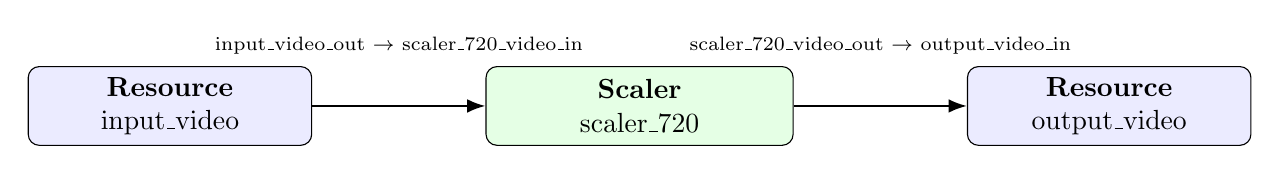
\begin{tikzpicture}[
  node distance=22mm,
  >=Latex,
  flow/.style={draw, rounded corners, minimum width=3.6cm, minimum height=1.0cm, align=center, fill=blue!8},
  proc/.style={draw, rounded corners, minimum width=3.9cm, minimum height=1.0cm, align=center, fill=green!10},
  arr/.style={->, thick}
]
  \node[flow] (in) {\textbf{Resource}\\input\_video};
  \node[proc, right=of in] (scaler) {\textbf{Scaler}\\scaler\_720};
  \node[flow, right=of scaler] (out) {\textbf{Resource}\\output\_video};

  \draw[arr] (in) -- node[above, font=\scriptsize, yshift=15pt]{input\_video\_out $\rightarrow$ scaler\_720\_video\_in} (scaler);
  \draw[arr] (scaler) -- node[above, font=\scriptsize, yshift=15pt]{scaler\_720\_video\_out $\rightarrow$ output\_video\_in} (out);
\end{tikzpicture}
}
\end{frame}

\begin{frame}{Visualisasi \texttt{flow2.model}: Pipeline Bercabang}
\vspace{8pt}
\centering
\scalebox{0.72}{
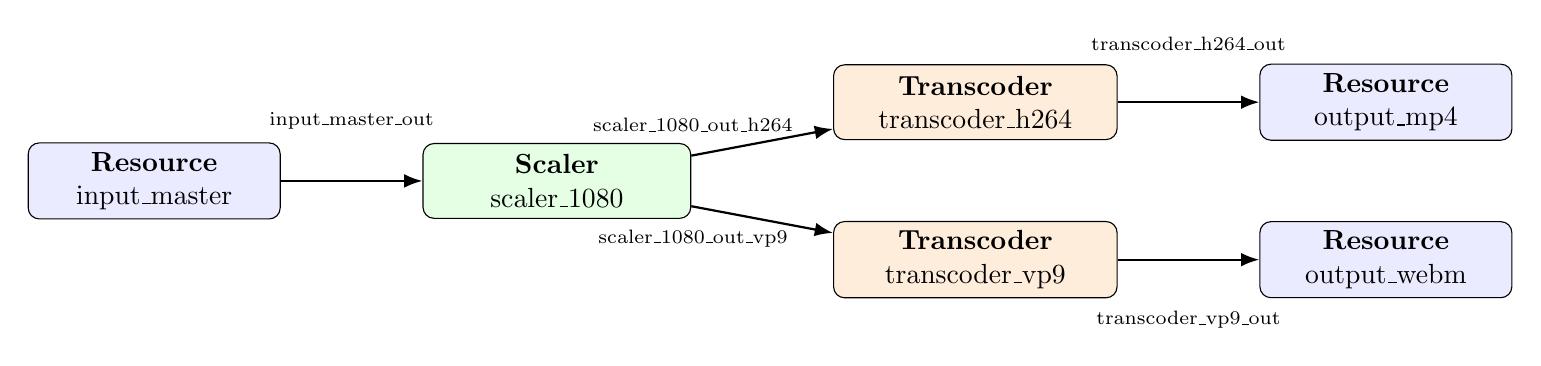
\begin{tikzpicture}[
  node distance=18mm and 18mm,
  >=Latex,
  res/.style={draw, rounded corners, minimum width=3.2cm, minimum height=0.95cm, align=center, fill=blue!8},
  scl/.style={draw, rounded corners, minimum width=3.4cm, minimum height=0.95cm, align=center, fill=green!10},
  trn/.style={draw, rounded corners, minimum width=3.6cm, minimum height=0.95cm, align=center, fill=orange!14},
  arr/.style={->, thick}
]
  \node[res] (input) {\textbf{Resource}\\input\_master};
  \node[scl, right=of input] (scaler1080) {\textbf{Scaler}\\scaler\_1080};
  \node[trn, right=of scaler1080, yshift=10mm] (h264) {\textbf{Transcoder}\\transcoder\_h264};
  \node[trn, right=of scaler1080, yshift=-10mm] (vp9) {\textbf{Transcoder}\\transcoder\_vp9};
  \node[res, right=of h264] (outmp4) {\textbf{Resource}\\output\_mp4};
  \node[res, right=of vp9] (outwebm) {\textbf{Resource}\\output\_webm};

  \draw[arr] (input) -- node[above, font=\scriptsize, yshift=15pt]{input\_master\_out} (scaler1080);

  \draw[arr] (scaler1080) -- node[above, font=\scriptsize, xshift=-25pt]{scaler\_1080\_out\_h264} (h264);
  \draw[arr] (scaler1080) -- node[below, font=\scriptsize, xshift=-25pt]{scaler\_1080\_out\_vp9} (vp9);

  \draw[arr] (h264) -- node[above, font=\scriptsize, yshift=15pt]{transcoder\_h264\_out} (outmp4);
  \draw[arr] (vp9) -- node[below, font=\scriptsize, yshift=-15pt]{transcoder\_vp9\_out} (outwebm);
\end{tikzpicture}
}
\end{frame}

\section{Ringkasan}
\begin{frame}{\hfill}
	\centering
	\Huge{\textbf{Ringkasan}}
\end{frame}

\begin{frame}{Kesimpulan Sesi}
\vspace{6pt}
\begin{itemize}
  \item MDSE menempatkan model sebagai artefak utama pengembangan.
  \item Konsep metamodel, model, instance, transformasi, dan validasi membentuk alur terintegrasi.
  \item Studi kasus MediaFlow menunjukkan satu metamodel mendukung variasi pipeline linear dan bercabang.
  \item Representasi tekstual (YAML/DSL) dan visual memudahkan authoring, review, dan komunikasi desain.
  \item Pendekatan MDSE membantu mengelola kompleksitas dan menjaga konsistensi implementasi.
\end{itemize}
\end{frame}

\end{document}
